\section{Metodología de trabajo y planificación del proyecto}
\subsection{Metodología de trabajo}
Inicialmente se planteó una metodología de trabajo inspirada en el modelo de ciclo de vida del software
basado en prototipos. Siendo el prototipo una aplicación con al menos una funcionalidad implementada,
que se le presentará al cliente con la que podrá ver los avances y como se resuelve el requisito planteado.
Además este podrá dar su opinión al respecto permitiendo modificar la forma en la que se implementa si no
es lo esperado o no se ajusta con lo que había previsto, con ello se esperaba obtener un software a
medida que se ajustara de la mejor forma posible a las problemáticas.

\medskip
Una vez realizada la primera reunión con el cliente y planteada la metodología prevista este lo consideró
inviable, puesto que no tiene la disponibilidad necesaria para hacer reuniones con frecuencia y probar el
resultado obtenido hasta ese momento. Por ello hubo que cambiar la metodología a una clásica en cascada,
esta consiste en plantear las tareas de manera secuencial e ir solucionando cada una solamente después de
haber terminado la anterior. Una vez se ha concluido con todas, ya tendremos nuestro proyecto finalizado
y listo para presentar y validar.

\medskip
Se ha decidido utilizar finalmente esta metodología al ser la que mejor se ajusta a las necesidades del
cliente y por la fuerte dependencia entre las funcionalidades. Puesto que la mayoría necesitan de que
exista previamente otra.

\subsection{Planificación inicial del proyecto}
Tras un estudio del estado del arte actual, se decidió en la primera fase del proyecto hacer un análisis
de la problemática con el que decidir cuales son los actores que intervienen en el sistema, es decir,
cuales serán los usuarios que interactuarán con él y que funcionalidades podrán usar cada uno. Estas
funcionalidades también se decidirán en esta primera fase de análisis. Para todo ello se hará uso de
de los diagramas de casos de uso \cite{casos-de-uso} y las tablas de especificación de los casos de
uso \cite{tabla-especificacion-casos-de-uso}.

\medskip
Una vez se decidió los actores que actúan en el sistema y los requisitos (funcionalidades) de cada uno
se continuó con un prototipo de la interfaz, para poder tener una primera visualización de los objetivos
que se tenía con esta aplicación.

\medskip
Este prototipo fue de gran ayuda puesto que se solucionaron dudas que había en ese momento sobre
las funcionalidades planteadas y las soluciones propuestas, además planteó otras dudas sobre otros requisitos
que no se habían planteado en un primer momento. A continuación se comentarán el cambio más significativo.

\medskip
Inicialmente en la primera pantalla de los pacientes, se usó una lista con una imagen del ejercicio y el
título de este como se puede ver en la figura \ref{patient-home-v1}. Tras la presentación de este primer prototipo,
se decidió que estas ocupaban demasiado espacio en la pantalla y eran molestas. Es por ello que se pasó a mostrar los
ejercicios solamente con el título.

\begin{figure}[!h]
    \centering
    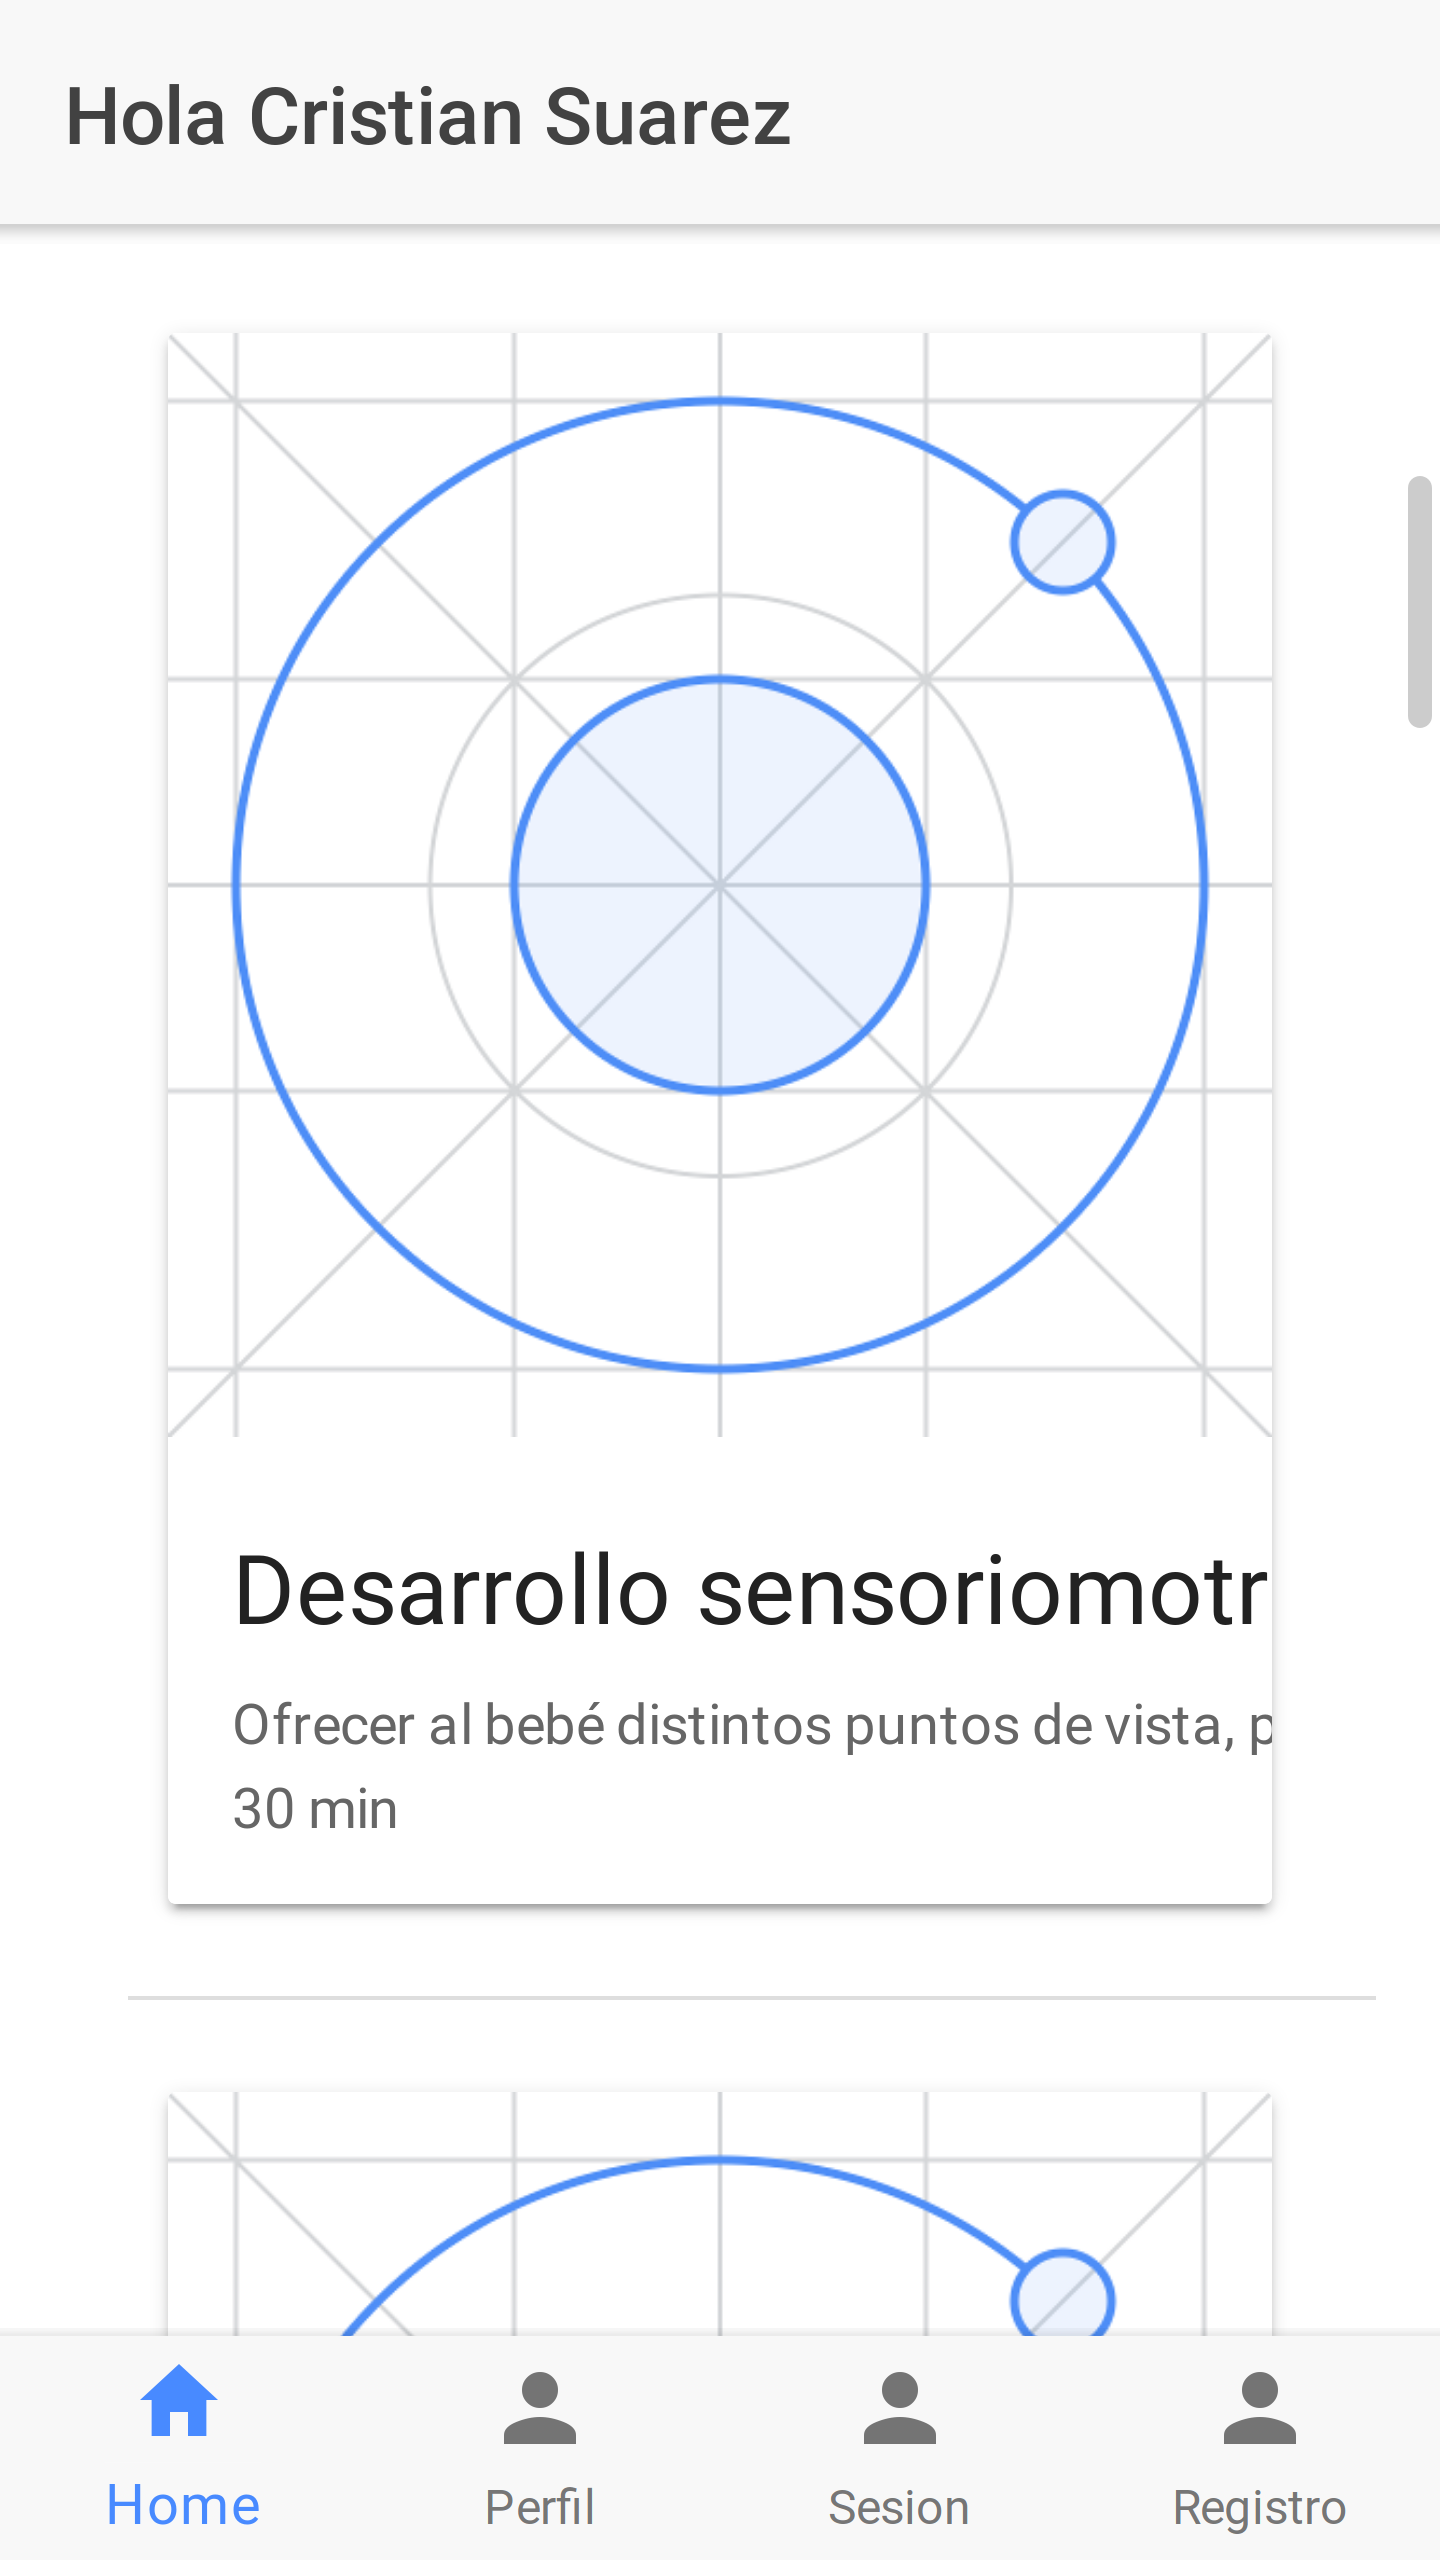
\includegraphics[width=0.5\textwidth]{images/screenshots/patient-home-v1.png}
    \caption{Pantalla inicial paciente, prototipo}
    \label{patient-home-v1}
\end{figure}


\medskip
Con esa parte ya solventada se empezó con el aprendizaje de la tecnología a usar, \textit{Ionic} \cite{ionic}.
Para el aprendizaje de este \textit{framework} se hizo una pequeña aplicación de gestión de tareas
sugerida en el propio libro de aprendizaje utilizado, \textit{"Learning ionic : buid hybrid mobile
applications with HTML5"} \cite{ionic-book}. Para complementar el aprendizaje de este libro se realizó
varios tutoriales \textit{online}, con todo ellos se adquirió experiencia y fluidez en el uso del
\textit{framework}.

\medskip
Una vez acabada la fase de aprendizaje se continuó con el desarrollo, este contemplaba las funcionalidades
que se describirán a continuación:

\medskip
\textbf{Las comunes para todos los usuarios:}
\begin{enumerate}
    \item Registro e inicio de sesión
    \item Vista del perfil personal
    \item Editar el perfil
    \item Enviar y reproducir vídeos
    \item Ver ejercicios
\end{enumerate}

\medskip
\textbf{Específicas del paciente:}
\begin{enumerate}
    \item Marcar ejercicio como hecho
\end{enumerate}

\medskip
\textbf{Específicas del doctor:}
\begin{enumerate}
    \item Buscar paciente
    \item Asignar ejercicio
    \item Añadir observaciones al ejercicio que se va a asignar
    \item Ver el perfil de un paciente
    \item Ver la evolución de un paciente
\end{enumerate}

\subsection{Ajustes en la planificación del proyecto}
En la tabla 1 se muestra de forma resumida la planificación inicial del proyecto, donde
podemos ver las principales fases y tareas y una estimación de las horas de trabajo
previstas para cada una de ellas. Sin embargo, la tarea de implementación (\textbf{Tarea 2.4})
se tuvo que retrasar según lo previsto inicialmente,
puesto que la tarea de aprendizaje (\textbf{Tarea 2.3}) del \textit{framework} llevó más de lo esperado.
A ello hay que añadirle que se decidió incorporar una funcionalidad que no se esperaba realizar,
la referente con la creación de un chat paciente - doctor y todo lo que ella conlleva, porque se
consideró que esta sería la forma más intuitiva para el usuario de enviar vídeos. Esto hizo que además
de retrasarse la implementación aumentase el tiempo que requiere. Es por todo ello que
dentro de la fase de diseño e implementación la distribución de tiempo entre tareas no fue el esperado.
Y finalmente la última funcionalidad referente al envío de vídeos no se pudo completar al cien por cien.

\medskip
En la siguiente tabla \ref{planificacion-inicial} se muestran la planificación inicial del proyecto.
\begin{table}
    \begin{tabular}{|lp{12cm}|}
        \hline
        FASES (HORAS) & TAREAS \\ \hline

        \multirow{3}{*}{Análisis}
        \multirow{3}{*}{(70)}
        & Tarea 1.1: Estudio del problema y soluciones actuales \\
        & Tarea 1.2: Captura de los requisitos del sistema \\
        & Tarea 1.3: Prototipo de la interfaz de usuario del sistema \\ \hline

        \multirow{4}{*}{Diseño}
        \multirow{4}{*}{(160)}
        & Tarea 2.1: Diseño de la estructura del sistema \\
        & Tarea 2.2: Diseño de la base de datos \\
        & Tarea 2.3: Aprendizaje de tecnologías de implementación: Ionic 2, etc \\
        & Tarea 2.4: Implementación de prototipos de la aplicación móvil \\ \hline

        \multirow{2}{*}{Pruebas}
        \multirow{2}{*}{(30)}
        & Tarea 3.1: Pruebas de funcionamiento de la aplicación móvil \\
        & Tarea 3.2: Pruebas de integración y rendimiento de la aplicación móvil \\ \hline

        \multirow{2}{*}{Documentación}
        \multirow{2}{*}{(40)}
        & Tarea 4.1: Realización de la memoria \\
        & Tarea 4.2: Realización de la presentación del TGF \\ \hline
    \end{tabular}

    \caption{Tabla planificación inicial del proyecto.}\label{planificacion-inicial}
\end{table}